%************************************************
\chapter{Resilience}\label{ch:resilience}
%************************************************
Topic 4: Write a brief introduction to Resilience in microservice architectures and to how Gatling load testing framework can be used for testing. Run load testing scenarios against the handed out containers and describe the effects of using patterns.
- run different load testing scenarios handed out
- hand-in generated reports and key metrics on BlackBoard 
- hand in exercise report
- run load-testing against your project architecture to see the effects

The word resilience mean "The capacity to recover quickly from difficulties". there are many definitions of the resilience, one of the definitions is taken from the book "The Resilience of Networked Infrastructure Systems". Fiskel (2003) defines a resilient system as a system that has the ability to return to a stable equilibrium state after a perturbation. 

There are different categories of potential disruptions to system that create the need to implement the resilience in systems. In the figure \ref{ch:resilience} below the sources of disruptions is showed. 

\begin{itemize}
	\item Human Factor
	\begin{itemize}
		\item UNDER
	\end{itemize}
	\item Natural Factors
	\begin{itemize}
		\item dfrgh
	\end{itemize}
	\item Organizational factors
	\begin{itemize}
		\item dfghdfsgh
	\end{itemize}
	\item Technical Factors
	\begin{itemize}
		\item dfrgh
	\end{itemize}
	
	
\end{itemize}



\begin{figure}[bth]
	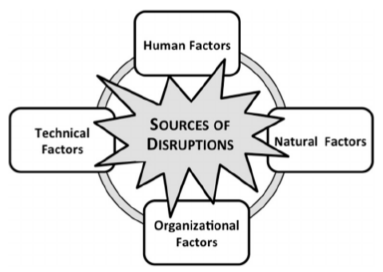
\includegraphics[width=0.7\linewidth]{gfx/resilience}
	\caption[routingtable]{Sources of disruptions} \label{fig:resilience}
\end{figure}   
